\chapter{Results and Evaluation}

\section{EDB Analysis}\label{edb analysis}
  A substantial part of my work was the exploitation of available sources, namely the EDB and the scraped epidemiological news. In the following I introduce how I recovered most of the information in the EDB for my further analyzes and how I managed to scrape a large amount of epidemiological data with a limited time profile.

\subsection{Source Determination}
  Before I could train a classifier to detect relevant articles or extract meaningful key words from texts, I needed to create a labeled dataset from the EDB. Therefor, I collected all articles that were read by the epidemiologists but were not put into the EDB. However, writing a script for information retrieval (such as scraping) can be time consuming so I needed to narrow down the, at that moment, 75 sources used in the EDB.

  The decision which source to extract was then made by the relevance and the complexity to retrieve information from this source.
  First, I extracted all URLs from the EDB and clustered them based on their netloc (a first level domain such as www.rki.de) to rank the URLs used in the EDB (Fig. \ref{fig:netloc}) to then only focus on sources frequently used. Then, I pinpointed those sources that are the most accessible. To do so, I evaluated the INIG reading checklist which includes all sources that are mandatory to observe. In this evaluation, I determined the data type, conducted exemplary information extractions to determine the accessibility, and evaluated the relevance of these sources by their articles(Fig. \ref{table:INIGsources}). Generally, information extraction from the INIG reading checklist was more difficult for PDF and Emails. PDFs, unlike HTML, do not consist of an markup language were certain information can specifically be extracted. Emails, on the other hand, were difficult to get access to due to privacy reasons and the information in them was usually less structured.

\begin{figure}
  \centering
  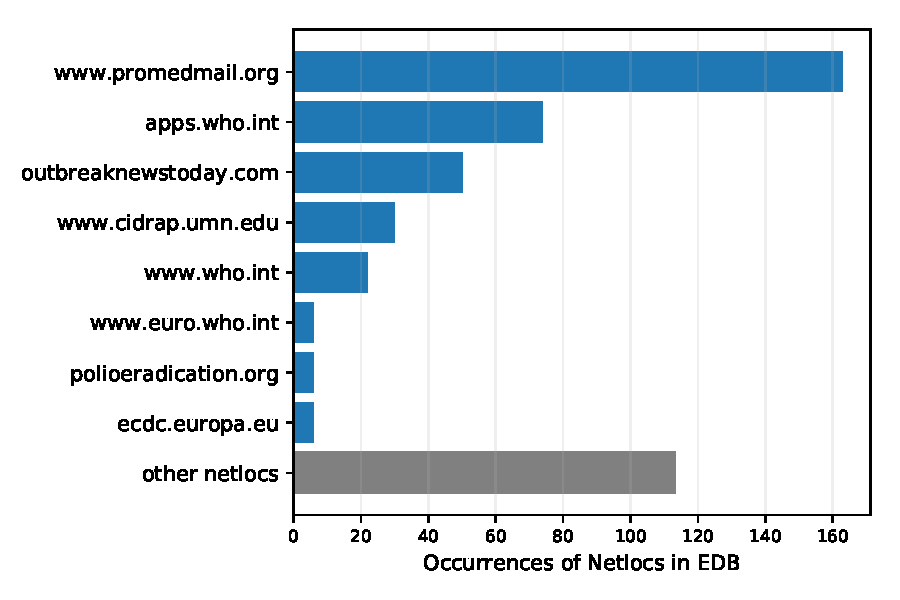
\includegraphics[scale=0.8]{netloc.pdf}
  \caption{The netfloc frequency of the most used sources of the EDB. Shown in grey is the sum of EDB entries referencing the other 67 netlocs not shown in this figure.}
\label{fig:netloc}
\end{figure}


\begin{table}
  \centering
  \begin{tabular}{@{}cccc@{}}
    \toprule
    \textbf{Source} & \textbf{Data Format} & \textbf{Data Quality} & \textbf{Accesibility}\\
    \midrule
    \href{http://www.cidrap.umn.edu/}{CIDRAP} & HTML & Mixed content & Intermediate \\
    \href{http://www.promedmail.org/}{ProMED Mail} & HTML & Only relevant & Easy\\
    \href{http://www.who.int/csr/don/en/}{WHO DONs} & HTML & Only relevant & Easy \\
    EIOS daily digest & Email & Only relevant & Hard \\
    \href{http://outbreaknewstoday.com/}{OutbreakNewsToday} & HTML & Mixed content & Intermediate\\
    ECDC Report & Email & Only relevant & Hard \\
    \href{http://www.afro.who.int/fr/health-topics/disease-outbreaks/outbreaks-and-other-emergencies-updates}{WHO Afro Bulletin} & PDF & Only relevant & Hard \\
    \href{http://www.eurosurveillance.org/content/eurosurveillance/browse}{EuroSurveillance} & PDF and HTML & Mixed content & Intermediate \\
    \href{http://www.who.int/wer/en/}{WHO WER} & PDF & Mixed content & Hard\\
    \href{https://ecdc.europa.eu/en/threats-and-outbreaks/reports-and-data/weekly-threats}{ECDC CDTR} & PDF & Only relevant & Intermediate \\
    \href{http://www.emro.who.int/pandemic-epidemic-diseases/information-resources/weekly-epidemiological-monitor.html}{WHO EMRO} & PDF & Mixed content & Hard \\
    \href{https://www.paho.org/hq/index.php?option=com_content&view=article&id=14044:epidemiological-alerts-archive-by-year-2018&Itemid=72203&lang=en}{WHP PAHO} & PDF & Only relevant & Intermediate\\
    \bottomrule
  \end{tabular}
  \caption{An evaluation of the INIG reading checklist by source, data quality and accessibility. The data format refers to the final data format of the epidemiological text. The data quality describes whether a source only contain information relevant for epidemiological surveillance or also research findings and ongoing projects (mixed content). The difficulty evaluation is based on exemplary information retrieval from these sources where \textsl{easy} posed no difficulty, \textsl{intermediate} would have required additional work but was promising to function and \textsl{hard} was unsure whether it could work satisfactorily.}
  % \setlength{\tabcolsep}{1.5em}
\label{table:INIGsources}
\end{table}

\subsection{Data Quality}
  Due to the unrestrained column settings, every entry in the EDB was free text with spelling mistakes and different formatting. The transferral of the EDB into a controlled vocabulary, as described in \ref{controlled vocabulary}, was a vital steps since it made more data points useable. Tab. \ref{table:preprocessing performance} shows that the preprocessing made up around 100 EDB entries accessible per keyword.

\begin{table}
  \centering
  \caption{A performance measure of the transmission of the EDB data to a controlled vocabulary. The key word were the columns found in the EBD with the amount of valid entries before and after the preprocessing out of 557 entries. Note, although the date validity numbers did not change after preprocessing, the dates underwent an important preprocessing step from a string to a timestamp object to allow computation on them.}
  \begin{tabular}{@{}cccc@{}}
    \toprule
    \textbf{Key Word} & \textbf{Valid Before} & \textbf{Valid After} & \textbf{Invalid After} \\
    & \textbf{Preprocessing} & \textbf{Preprocessing} & \textbf{Preprocessing} \\
    \midrule
    Date& 168 (30\%)& 168(30\%)&  19 (3\%) \\
    Case count& 299 (54\%)& 394 (71\%)&  18(3\%) \\
    Country& 355 (64\%)& 494 (88\%)&  17(3\%) \\
    Disease& 231 (41\%)& 332 (60\%)& 16(3\%) \\
    \bottomrule
  \end{tabular}
\label{table:preprocessing performance}
\end{table}

\subsection{Evaluation}
  The focused preprocessing of the EDB and the assembly of a training data set was successful. With only two scraper, I was able to use half of the entries of the EDB to create a labeled dataset by analyzing the usage frequency (Fig. \ref{fig:netloc}), accessibility, and relevance of the source (Fig . \ref{table:INIGsources}). This dataset, then was even further preprocessed which retrieved around 100 data points per entity \ref{table:preprocessing performance}).

\section{Key Information Extraction}
  Although, EpiTator extracted only relevant entity classes, they still needed to be filtered for the key entity of this class, i.e., those that need to be put into the EDB.
  To do so, I used the most often occurring entity in one entity class, for example, the most frequent disease in one text (Lis. \ref{lst:mostoccure}).

  This worked well for the key information extraction of disease and country entities. Except for one occurrence of a disease that was not recognized by EpiTator, all countries and disease were detected correctly. However, this approach did not detect the correct key information of count and date entities.
  Thus, I trained multinomial and Bernoulli naive Bayes classifier using all sentences of a text containing a specific entity class. The label \emph{is key} was given to those sentences where the extracted entity matched the entity found in the EDB for this text and \emph{is not key} to the others.

\subsection{Results}
  The performance of both classifier for the key information extraction of count entities is shown in Fig. \label{table:keyword_performance_counts} and for date entities in Fig. \label{table:keyword_performance_dates}. The corresponding ROC curves and their AUC values are shown in \ref{fig:roc_key}. Since, there were strong expectations which phrases indicated the mentioning of a key entity such as \dots \textit{``confirmed cases"} \dots or \dots \textit{`` cases \dots as of"}\dots, I retrieved those token that were are strong indicator for the \emph{is key} label (Tab. \ref{table:important_words}).

\begin{table}
  \centering
  \caption{The most important words during the classification of the NBC to detect the key entities Counts and Dates.}
  \begin{tabular}{@{}lcc@{}}
    \toprule
    \textbf{Entity Class}& \textbf{Word} & \textbf{Positive (\%)}\\
    \midrule
    \textbf{Counts}& variant& 31.1\\
    & poultry& 27.1\\
    & Laibin& 27.1\\
    & 42-year-old& 22.2\\
    & strains.& 19.2\\
    & province.Aug& 19.2\\
    & 13For& 19.2\vspace{2mm}\\
    \textbf{Dates}
    & worm& 6.0\\
    & occuring& 5.3\\
    & Nothern& 5.3\\
    & emerging& 5.3\\
    & patients& 4.5\\
    & South& 4.1\\
    & deaths& 3.9\\
    \bottomrule
  \end{tabular}
\label{table:important_words}
\end{table}

\begin{table}
  \ra{1.1}
  \caption{The performance evaluation of the count entity key information extraction. For each classifier and label, the precision (Pre.), recall (Rec.), specificity (Spec.), F1, index balanced accuracy (IBA), and support (Sup.) is given.}
  \centering
  \begin{tabular}{@{}rcccccccc@{}}
    \toprule
     & \textbf{Pre.} & \textbf{Rec.} & \textbf{Spec.}
    & \textbf{F1} &  \textbf{IBA}& \textbf{Sup} \\
    \midrule
    \textbf{Multinomial Naive Bayes}\\
    \emph{is not key}& 0.91& 1.00&  0.00& 0.95& 0.00& 446 \\
    \emph{is key}& 0.00& 0.00&  1.00& 0.00& 0.00& 43 \\
    Average/Total& 0.83& 0.91& 0.09& 0.87& 0.00& 489 \vspace{2mm}\\
    \textbf{Bernoulli Naive Bayes}\\
    \emph{is not key}& 0.93& 0.90&  0.24& 0.91& 0.23& 447 \\
    \emph{is key}& 0.18& 0.24&  0.90& 0.21& 0.20& 42 \\
    Average/Total& 0.86& 0.84& 0.29& 0.85& 0.23& 489 \vspace{2mm}\\
    \bottomrule
  \end{tabular}
\label{table:keyword_performance_counts}
\end{table}

\begin{table}
  \ra{1.1}
  \caption{The performance evaluation of the date entity key information extraction. For each classifier and label, the precision (Pre.), recall (Rec.), specificity (Spec.), F1, index balanced accuracy (IBA), and support (Sup.) is given.}
  \centering
  \begin{tabular}{@{}rcccccccc@{}}
    \toprule
     & \textbf{Pre.} & \textbf{Rec.} & \textbf{Spec.}
    & \textbf{F1} &  \textbf{IBA}& \textbf{Sup} \\
    \midrule
    \textbf{Multinomial Naive Bayes}\\
    \emph{Irrelevant}& 0.67& 1.00&  0.00& 0.80& 0.00& 26 \\
    \emph{Relevant}& 0.00& 0.00&  1.00& 0.00& 0.00& 27 \\
    Average/Total& 0.44& 0.67& 0.33& 0.53& 0.00& 39 \vspace{2mm}\\
    \textbf{Bernoulli Naive Bayes}\\
    \emph{Irrelevant}& 0.78& 0.93&  0.11& 0.85& 0.11& 30 \\
    \emph{Relevant}& 0.33& 0.11&  0.93& 0.17& 0.10& 9 \\
    Average/Total& 0.68& 0.74& 0.30& 0.69& 0.11& 39 \vspace{2mm}\\
    \bottomrule
  \end{tabular}
\label{table:keyword_performance_dates}
\end{table}

\begin{figure}
  \centering
  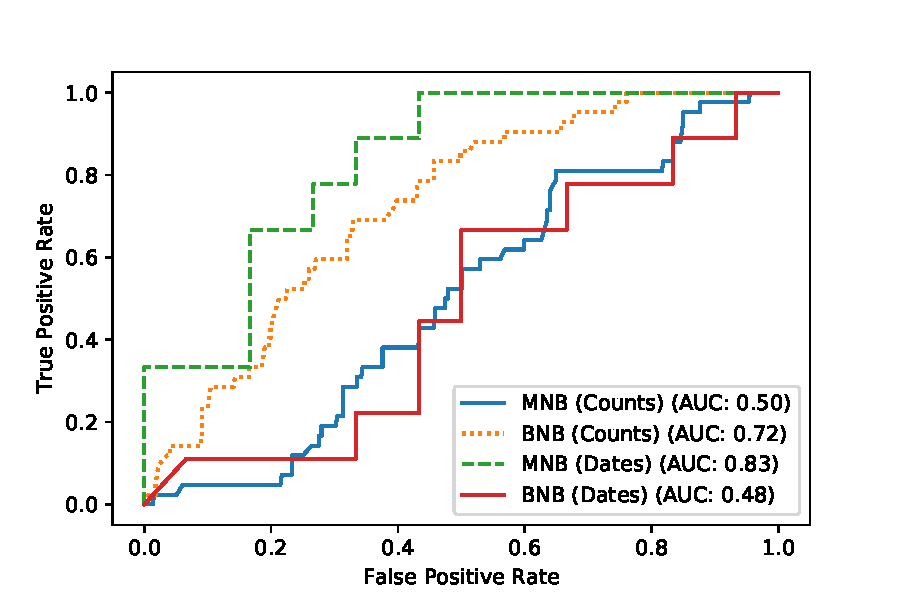
\includegraphics[scale=0.8]{roc_curves_key.pdf}
  \caption{A ROC-curve comparison of the different key information extraction classifier trained using a Multinomial naive Bayes (MNB) and Bernoulli naive Bayes (BNB) classifier with the respective value for the area under the curve (AUC).}
\label{fig:roc_key}
\end{figure}

\subsection{Evaluation}
  It is interesting that the multinomial naive Bayes was by a large margin better performing in the date entity selection from sentences than the Bernoulli naive Bayes. This finding contradicts the former expectation that Bernoulli naive Bayes is normally preferred in short text classifications. However, the opposite is true for the count entity recognition where the Bernoulli naive Bayes indeed is better, yet with a smaller difference. Nevertheless, both classifier were able to learn form the data, despite of their size (2445 data points in the count entity data set and 195 for the date entity data set). Surely, with more data that is put into a controlled database and not a free text Excel sheet, better results can be expected. Also, the words, most responsible for a positive classification (Tab. \ref{table:important_words}) were unlike the expectation to find words like \textit{confirmed} or phrases like \textit{as of}. Especially the count classification is based on poor tokenization (\textit{13For}, \textit{province.Aug}, and \textit{strains}). It looks better for the date classification and the word \textit{patients} or \textit{death} appear to make sense. Both words could be used in a sentence were the author would also place the date as of the confirmed case numbers are form.

\section{Article Recommendation}
  For the detection of relevant disease outbreak articles, I used the scraped WHO DONs and ProMED Mail articles together with the EDB entries, both of the year 2018, to built a labeled dataset. Since I intended to use also use word embeddings besides the bag-of-words approach to train a classifier, I visualized the word embeddings of the training data pretrained on the Wikipedia Corpus and Gigaword and self-trained embeddings using WHO DON and ProMED articles (Fig. \ref{fig:t-sne}). Finally, I compared classifier trained with the tf-idf transformed bag-of-word approach and document embeddings balanced with ADASYN shown in Tab. \ref{table:recommender_performance}.

\subsection{Results}
  The pretrained embeddings showed the typical clustering of similar tokens such as digits at the coordinates(-40, -90), names (-75,25), adjectives (50,-75), and medical terms at (0,25) (Fig. \ref{fig:t-sne}).
  But, the self-trained embeddings appear to cover more health-related terms from the center up to the upper right corner that seem to be clustering. Additionally, it also contains typical clusters such as digits (-20,30) (Fig. \ref{fig:t-sne}). However, most cluster are not specific enough but are rather a neighborhood.

  Since the primary goal of the trained classifier is the recognition of relevant articles, the recall for the \emph{relevant} label is important. Tab. \ref{table:recommender_performance} shows that the SVM has the highest score for recall of relevant articles. Also, the IBA is the highest in average for the support vector classifier which takes the class imbalance into account opposed to the F1 score. The CNN is the worst performing classifier in both these measures. The complement naive Bayes and multinomial naive Bayes classifier performed equally good.

\begin{figure}
  \centering
  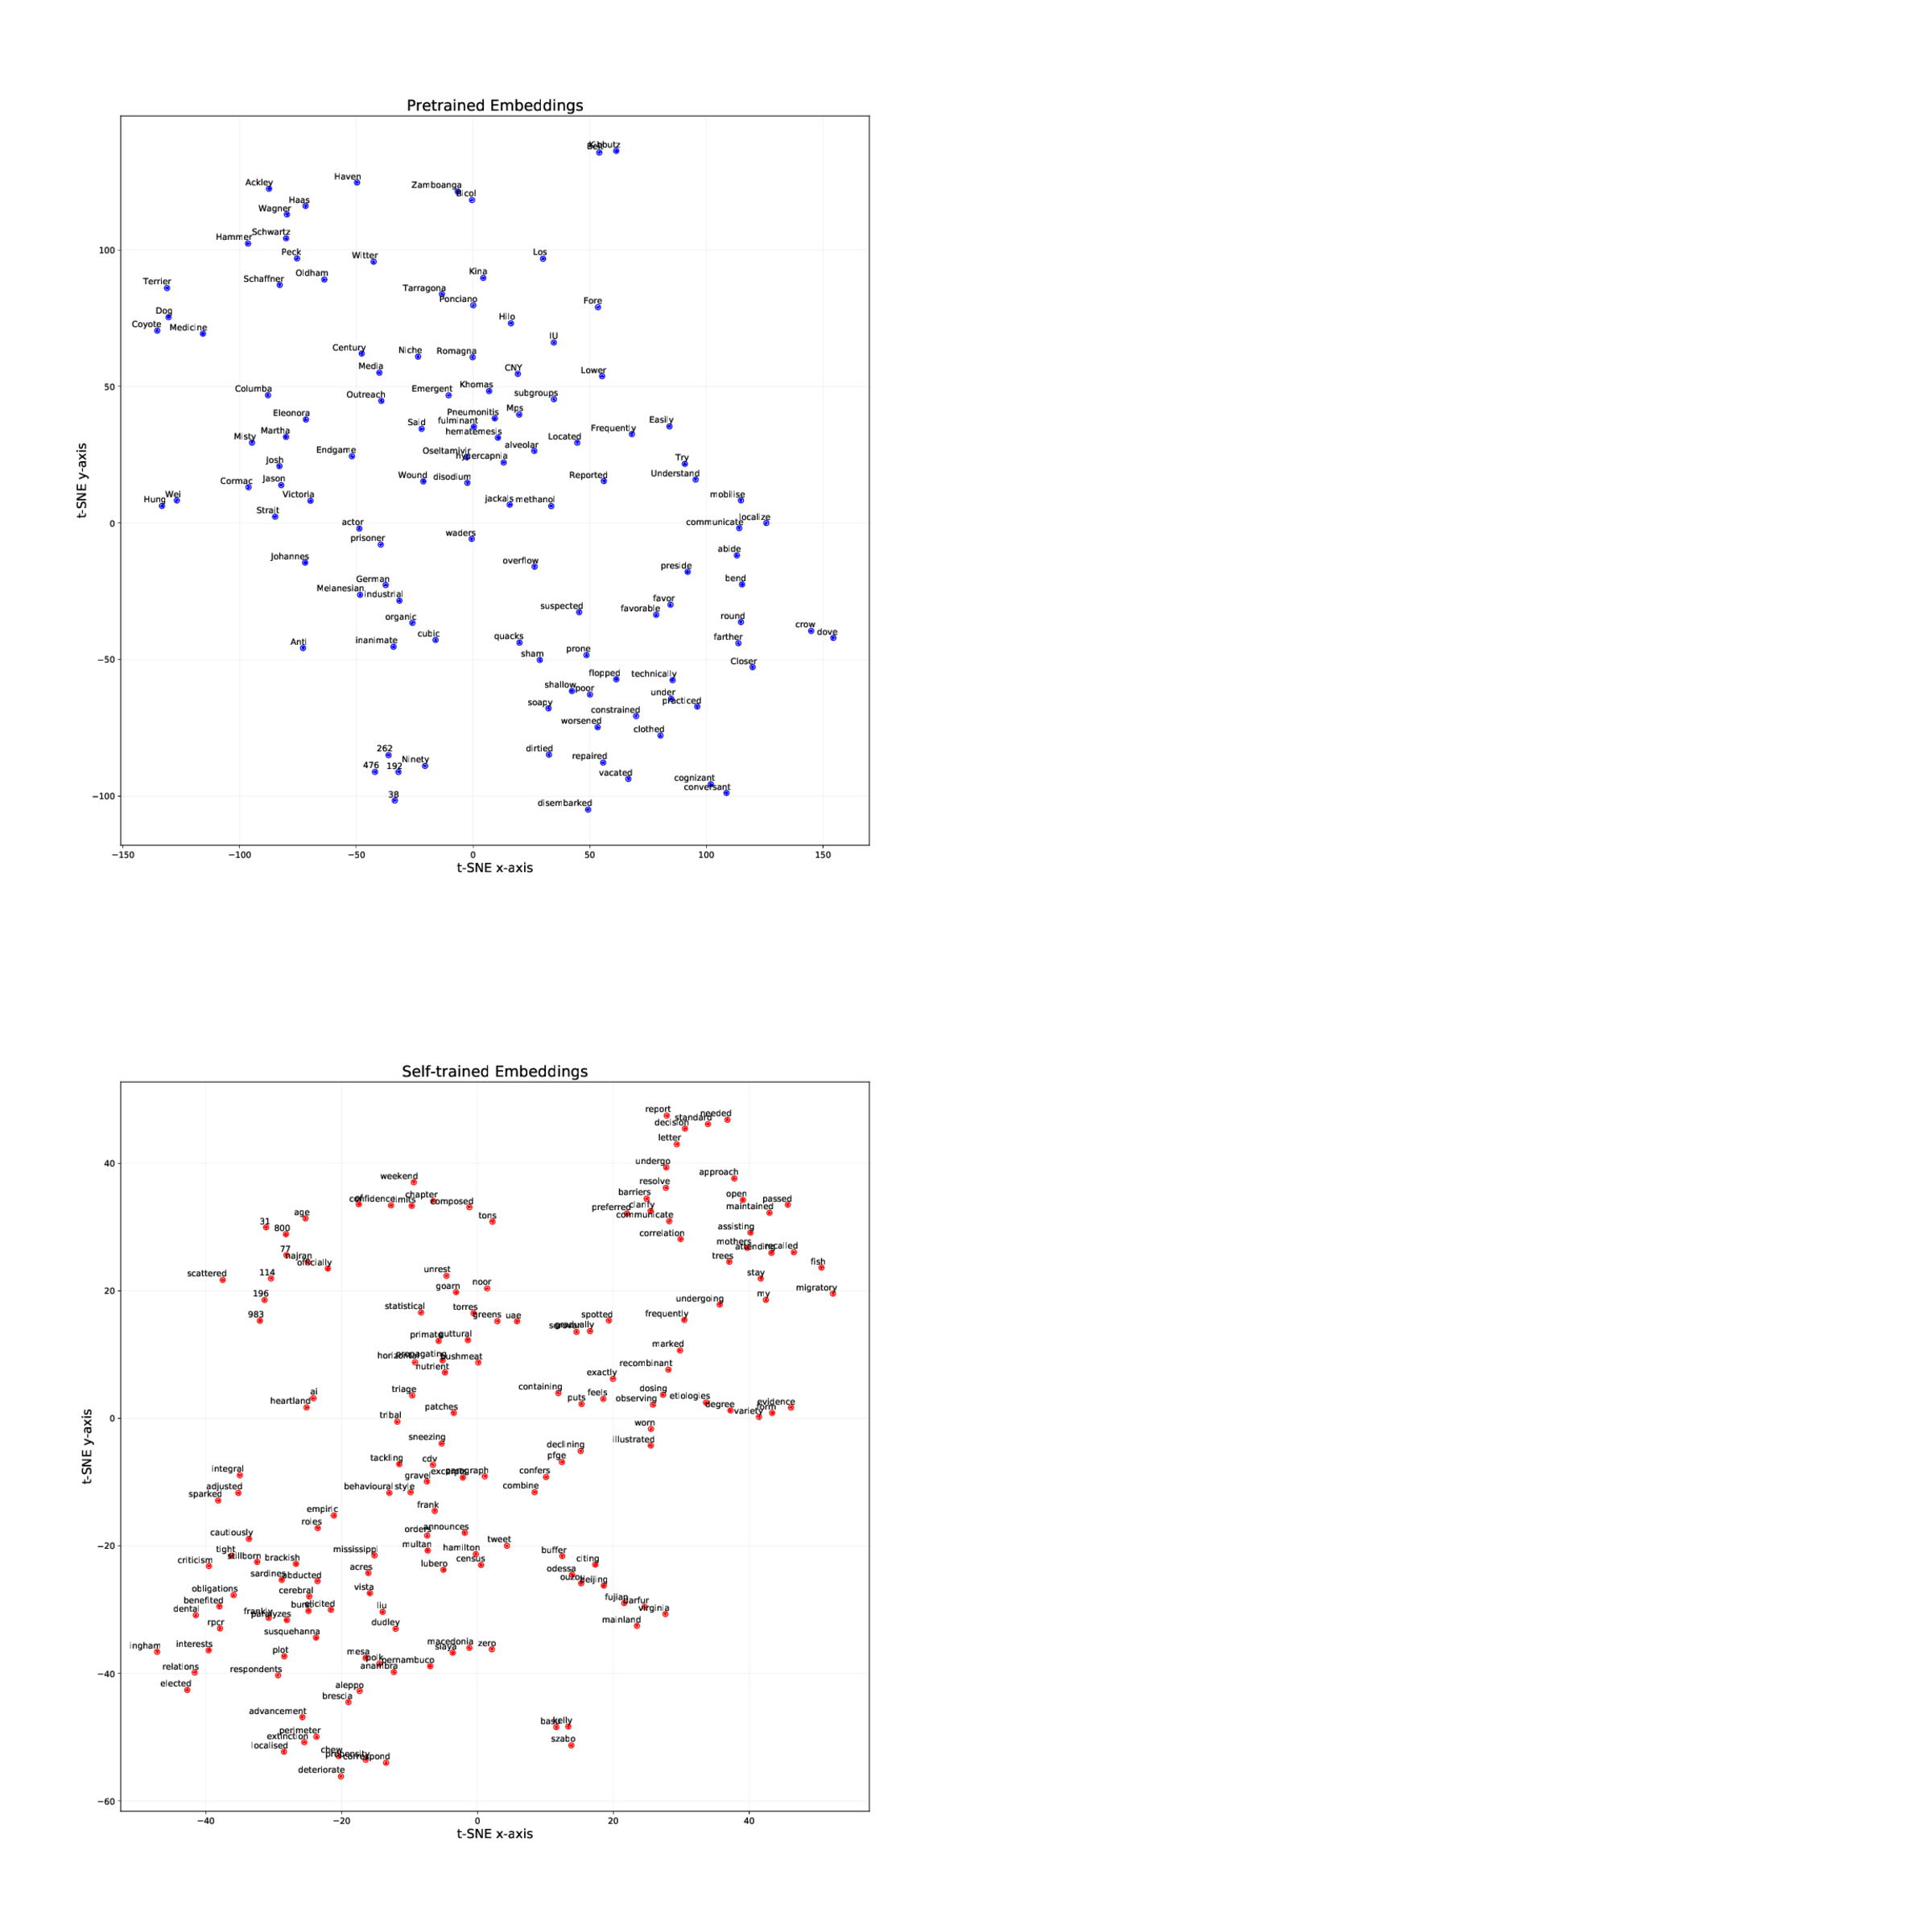
\includegraphics[scale=0.6]{t-sne-combined-v.pdf}
  \caption{A comparison of word embeddings applied to the training data using embeddings pretrained on the Wikipedia and Gigaword corpus (blue) and on WHO DON and ProMED articles (red) using t-SNE for dimensionality reduction.}
\label{fig:t-sne}
\end{figure}

\begin{table}
  \ra{1.1}
  \caption{The performance evaluation of the relevance classification. For each classifier and label, the precision (Pre.), recall (Rec.), specificity (Spec.), F1, index balanced accuracy (IBA), and support (Sup.) is given. The support vector classifier uses the radial basis function (RBF) as a kernel.}
  \centering
  \begin{tabular}{@{}rcccccccc@{}}
    \toprule
     & \textbf{Pre.} & \textbf{Rec.} & \textbf{Spec.}
    & \textbf{F1} &  \textbf{IBA}& \textbf{Sup} \\
    \midrule
    \textbf{Multinomial Naive Bayes}\\
    \emph{Irrelevant}& 0.96& 0.98&  0.10& 0.97& 0.11& 617 \\
    \emph{Relevant}& 0.21& 0.10&  0.98& 0.14& 0.09& 30 \\
    Average/Total& 0.92& 0.94& 0.14& 0.93& 0.11& 647 \vspace{2mm}\\
    \textbf{Complement Naive Bayes}\\
    \emph{Irrelevant}& 0.96& 0.98&  0,10& 0.97& 0.11& 617 \\
    \emph{Relevant}& 0.21& 0.10&  0.98& 0.14& 0.09& 30 \\
    Average/Total& 0.92& 0.94& 0.14& 0.93& 0.11& 647 \vspace{2mm}\\
    \textbf{Logistic Regression}\\
    \emph{Irrelevant}& 0.97& 0.67&  0.63& 0.79& 0.42& 762 \\
    \emph{Relevant}& 0.09& 0.63&  0.67& 0.15& 0.42& 38 \\
    Average/Total& 0.93& 0.66& 0.63& 0.76& 0.42& 800 \vspace{2mm}\\
    \textbf{K-Nearest Neighbor Classifier}\\
    \emph{Irrelevant}& 0.97& 0.77&  0.53& 0.86& 0.41& 762 \\
    \emph{Relevant}& 0.10& 0.53&  0.77& 0.17& 0.39& 38 \\
    Average/Total& 0.93& 0.75& 0.54& 0.82& 0.41& 800 \vspace{2mm}\\
    \textbf{Support Vector Machine (RBF)}\\
    \emph{Irrelevant}& 0.98& 0.60&  0.79& 0.74& 0.46& 762 \\
    \emph{Relevant}& 0.09& \textcolor{green}{0.79}&  0.60& 0.16& 0.48& 38 \\
    Average/Total& 0.94& 0.61& 0.78& 0.72& \textcolor{green}{0.47}& 800 \vspace{2mm}\\
    % \textbf{Support Vector Classifier (linear)}\\
    % \emph{Irrelevant}& 0.98& 0.65&  0.68& 0.78& 0.44& 762 \\
    % \emph{Relevant}& 0.09& 0.68&  0.65& 0.16& 0.45& 38 \\
    % Average/Total& 0.93& 0.65& 0.68& 0.75& 0.44& 800 \vspace{2mm}\\
    \textbf{Multi Layer Perceptron}\\
    \emph{Irrelevant}& 0.97& 0.78&  0.58& 0.87& 0.46& 762 \\
    \emph{Relevant}& 0.12& 0.58&  0.78& 0.19& 0.44& 38 \\
    Average/Total& 0.93& 0.77& 0.59& 0.83& 0.46& 800 \\
    \textbf{Convolutional Neural Network}\\
    \emph{Irrelevant}& 0.95& 1.00&  0.00& 0.98& 0.00& 762 \\
    \emph{Relevant}& 0.00& \textcolor{red}{0.00}&  1.00& 0.00& 0.00& 38 \\
    Average/Total& 0.91& 0.95& 0.05& 0.93& \textcolor{red}{0.00}& 800 \\
    \bottomrule
  \end{tabular}
\label{table:recommender_performance}
\end{table}

\begin{figure}
  \centering
  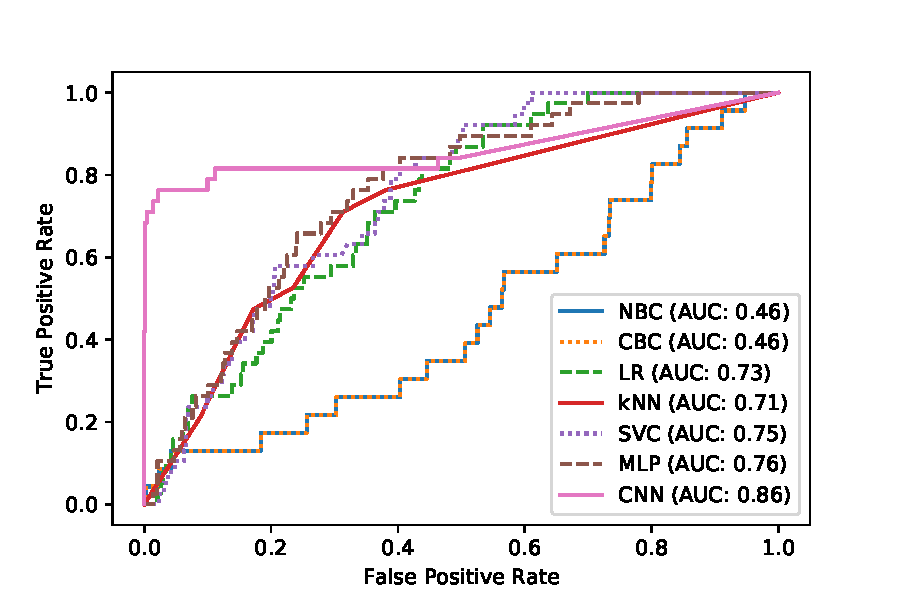
\includegraphics[scale=0.8]{roc_curves.pdf}
  \caption{A ROC-curve comparison of the different relevance classifier trained using a Multinomial naive Bayes (MNB), complement naive Bayes (CNB) classifier, logistic regression (LR), k-nearest neighbor classifier(kNN), support vector machine (SVM), multi layer perceptron (MLP) and convolutional neural network (CNN) with the respective value for the area under the curve (AUC). Note, the curves of the MNB and CNB overlay.}
\label{fig:roc_key}
\end{figure}

\subsection{Evaluation}
  It appears, that the pretrained word embeddings lacks the same amount of technical vocabulary as the self-trained embeddings. It is likely that a larger corpus containing the same specific language used in epidemiological news would yield a better foundation for training word embeddings and thus, a better classifier.

  Against expectations, the multinomial and complement naive Bayes both performed equally good, although the complement naive Bayes tackles problems occurring in imbalances datasets specifically. Also, the deep learning methods worked worked worse in respect of the imbalanced class measures and were only excelling regarding usual measures like the F1 score. A reason especially for the CNN might be, that it overfitted. This can be coped with dropout (removal of nodes in the network during training time), regularization (e.g. L2), and early stopping. However, building a well adjusted model was not in the scope of this thesis and requires a lot of time. Despite the results, I believe that with enough adjustments, the CNN could perform much better

\section{Web App}
  Finally, I built a web application using Flask and Datatables to visualize a possible workflow of the keyword extraction and relevance scoring (Fig. \ref{fig:t-aussinator}).

\subsection{Results}
  The web app allows the use to paste an URL for evaluation. The output of this processing is the extraction of keyword information of this article and a relevance score. The app is also allows a more automated workflow. The buttons \texttt{Get ProMED articles} or \texttt{Get WHO DONs} will trigger the automatic evaluation of all articles of the respective domain since the last evaluation. Instead of building an automated evaluation process, this function allows the user to observe the functionality of the application better. Furthermore, the application allows the extraction of the database with all evaluation in different data formats. That was an important step at this timepoint since INIG was not sure how to proceed to store data. Therefore, the app offers different possibilities to extract the database.

\begin{figure}
  \centering
  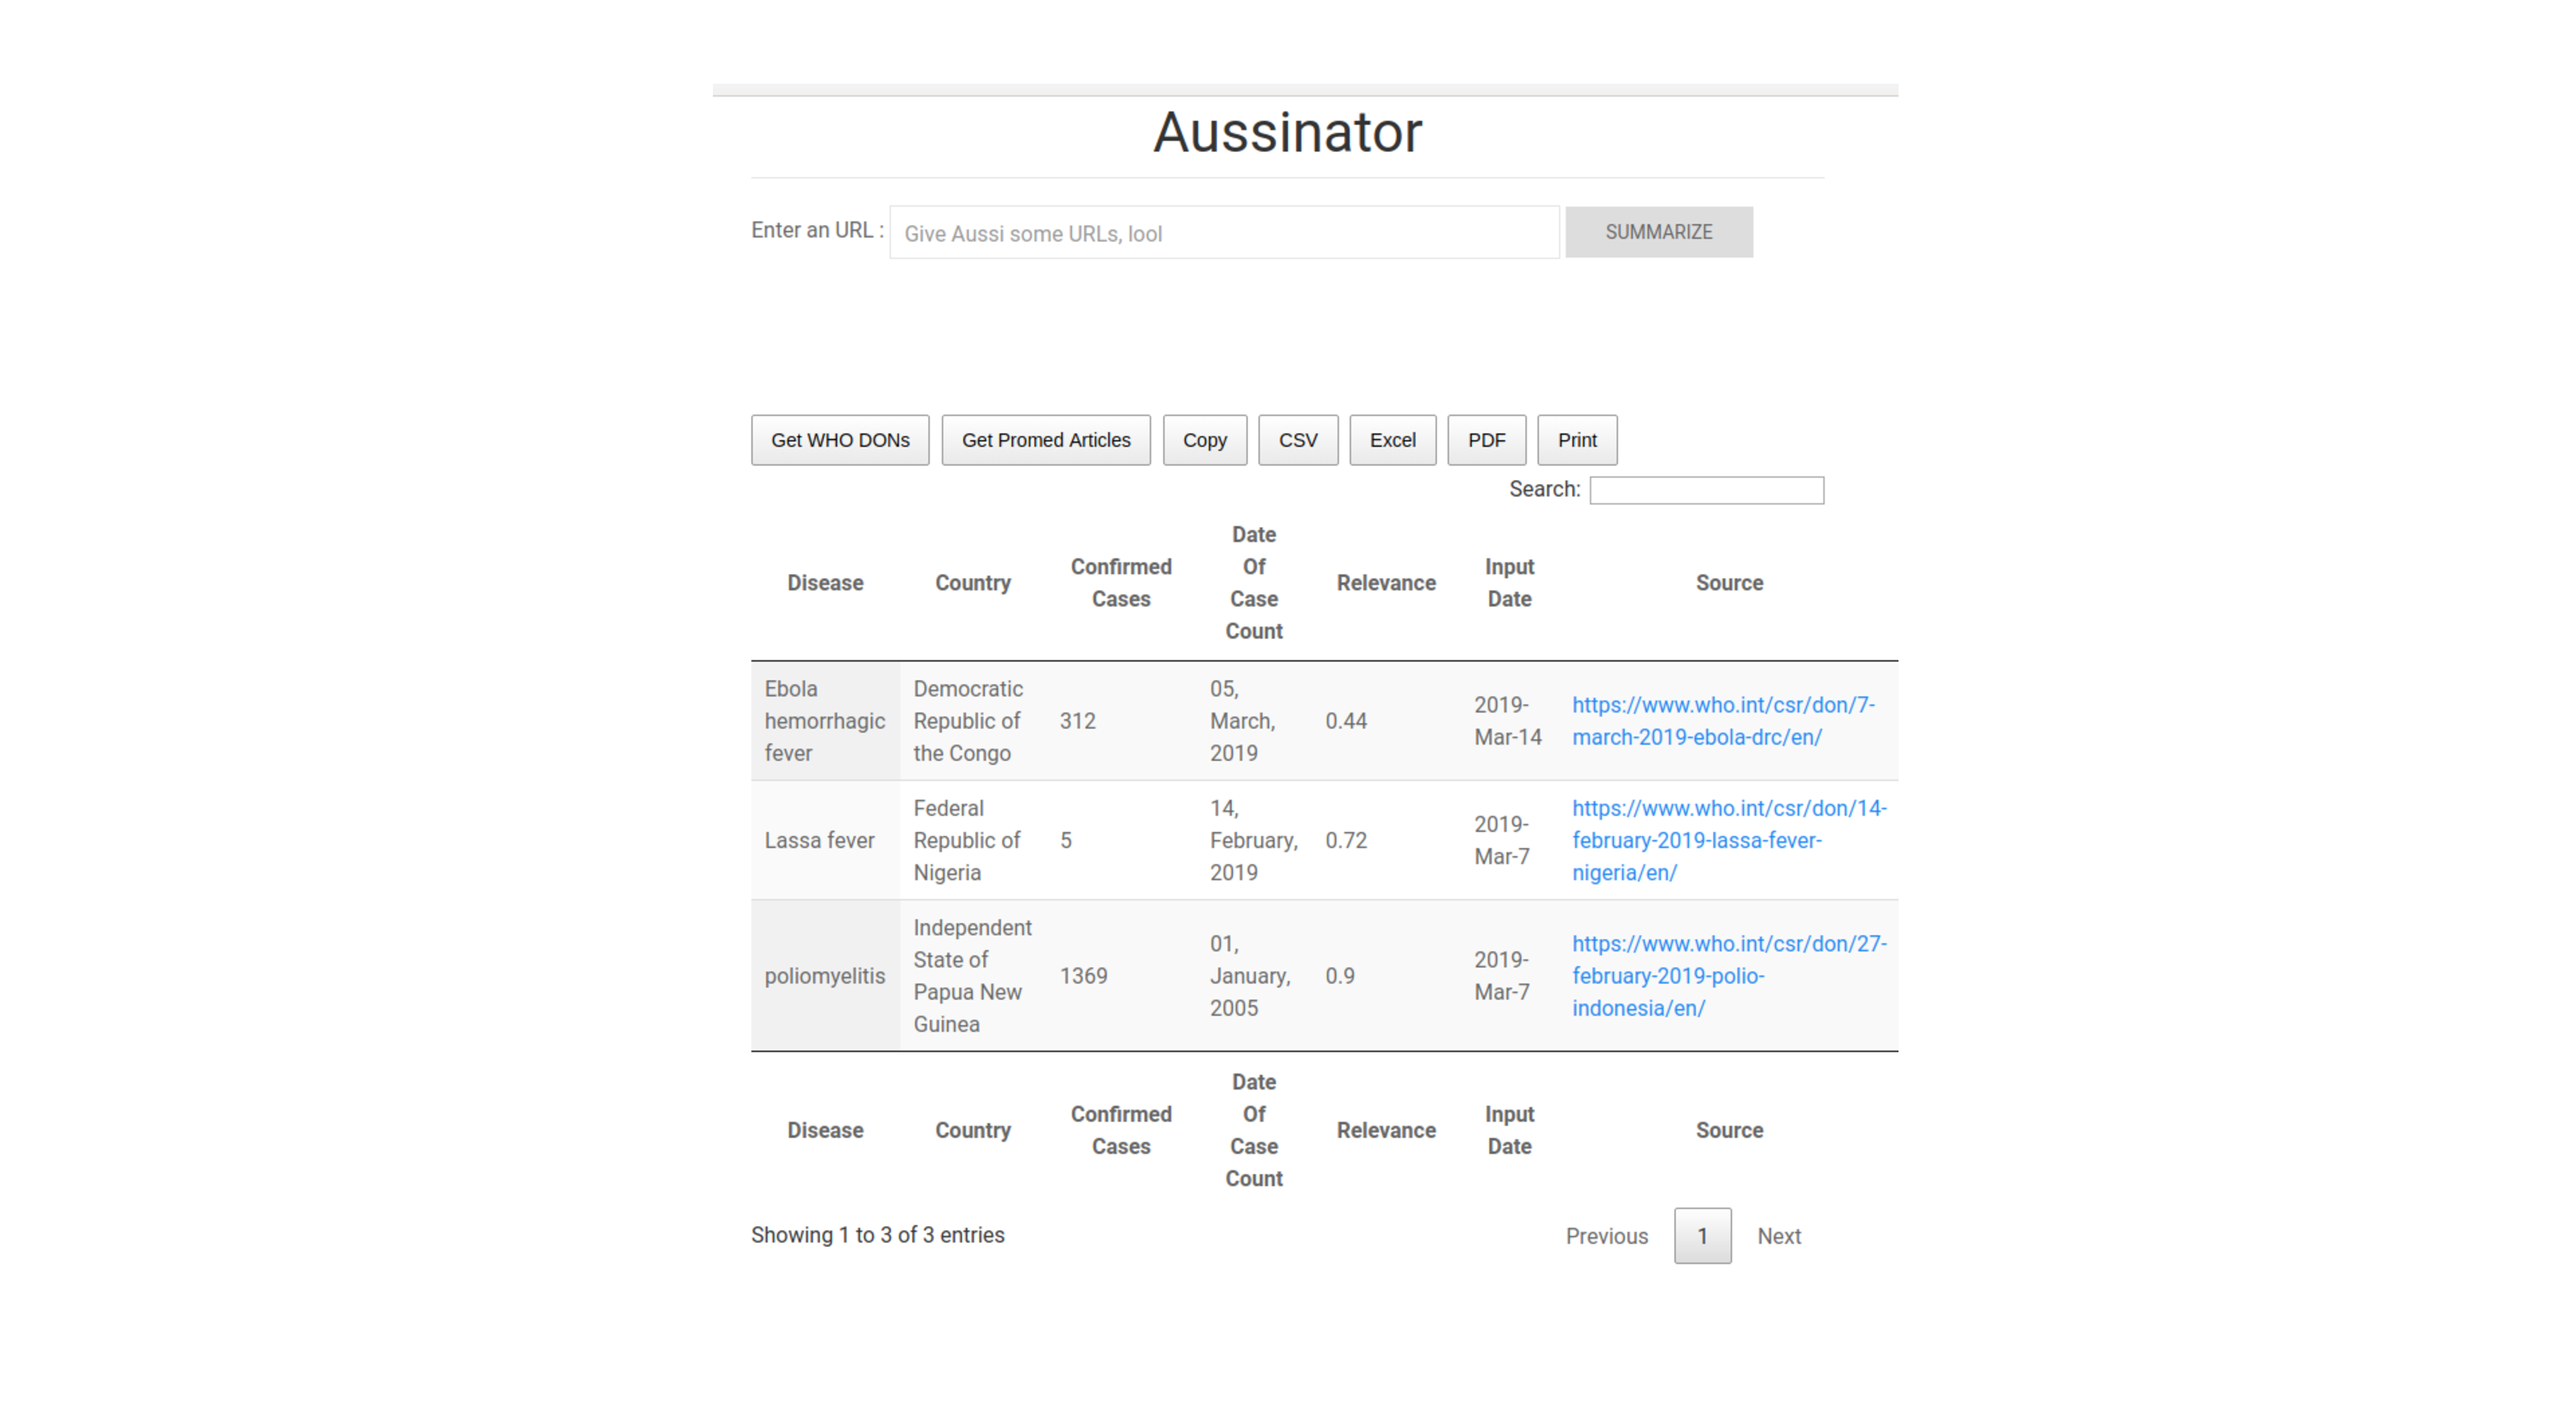
\includegraphics[scale=0.3]{aussinator.pdf}
  \caption{A Flask web application using the keyword extraction and relevance scoring trained as part of this thesis.}
\label{fig:t-aussinator}
\end{figure}

\subsection{Evaluation}
  Aussinator offers an easy access to the information extraction and relevance scoring developed during this thesis. Furthermore, it offers enough freedom during operation for the user who has a possibility to also validate the output of the app.
  However, the live extraction is rather slow. The processing of one URL takes one second and is noticeably too slow for spontaneous evaluations. This is particularly notable when extracting several articles as in intended by \texttt{Get ProMED articles}.
  The preprocessing by EpiTator is the bottleneck. NER usually takes some time, and EpiTator looks up for several entities which causes the delay.
  A solution would be a faster processor, which is however costly.
  Another solution to this would be a daemon process that regularly checks whether the sources in question published new articles.
  If so, it would then start evaluation this article and stores it in the background to increase the retrieval for the update functions \texttt{Get ProMED articles} and \texttt{Get WHO DONs}.
